\documentclass[9pt,aspectratio=169]{beamer}

% --- Theme ---
\usetheme{Singapore}
\setbeamertemplate{navigation symbols}{}   % no icons
\setbeamertemplate{mini frames}{}          % no dots in headline
\setbeamercovered{transparent}

% --- Grayscale colors ---
\definecolor{PelloGrayDark}{RGB}{60,60,60}
\definecolor{PelloGray}{RGB}{120,120,120}
\definecolor{PelloGrayLight}{RGB}{235,235,235}
\definecolor{PelloGrayUltraLight}{RGB}{248,248,248}

\usecolortheme[named=PelloGrayDark]{structure}

% --- Blocks ---
\setbeamertemplate{blocks}[rounded][shadow=false]
\setbeamercolor{block title}{fg=white,bg=PelloGrayDark}
\setbeamercolor{block body}{fg=black,bg=PelloGrayLight}
\setbeamercolor{block title example}{fg=white,bg=PelloGrayDark}
\setbeamercolor{block body example}{fg=black,bg=PelloGrayLight}
\setbeamercolor{section in head/foot}{fg=PelloGray,bg=PelloGrayLight}
\setbeamercolor{subsection in head/foot}{fg=PelloGray,bg=PelloGrayLight}
\setbeamercolor{frametitle}{fg=black}

% --- Itemize bullets (optional; keep if you like the style) ---
\setbeamertemplate{itemize item}{\raisebox{0.2em}{\scalebox{.6}{$\bullet$}}}
\setbeamertemplate{itemize subitem}{\raisebox{0.2em}{\scalebox{1}{$-$}}}

% --- Footer: frame numbers ---
\makeatletter
\setbeamertemplate{footline}{%
  \hfill\usebeamerfont{footline}\insertframenumber/\inserttotalframenumber\hspace{1em}\vspace{2pt}
}
\makeatother

% --- Minimal packages (add more only when needed) ---
\usepackage[english]{babel}
\usepackage[T1]{fontenc}
\usepackage[utf8]{inputenc}
\usepackage{graphicx}
\usepackage{tikz}
\usepackage{booktabs}
\usepackage{makecell} % for jumping lines within cells in tables.
\usepackage{multirow}
\usepackage{amsmath}
\usepackage{hyperref}
\hypersetup{colorlinks,linkcolor=,urlcolor=blue}
\usepackage{comment}
\usepackage{listings}
\lstset{
  language=R,
  basicstyle=\ttfamily\footnotesize,
  keywordstyle=\color{blue},
  commentstyle=\color{green!50!black},
  stringstyle=\color{red},
  frame=single,
  showstringspaces=false
}
\linespread{1.7}   % 1.0 = normal, 1.2–1.5 common
\AtBeginEnvironment{lstlisting}{\linespread{1}\selectfont} % keep code listings single-spaced

% --- Meta ---
\title{Applied Economics}
\subtitle{Scraping Data}
\author{Pello Aspuru}
%\institute{University of Vienna}
\date{Winter 2026/2027}

% --- Title page spacing + bottom-left author/date ---
\setbeamertemplate{title page}{
  \vspace{8em}
  \begin{center}
	{\usebeamerfont{title}\inserttitle\par}
  	\vspace{1.5em} % <-- increase title–subtitle gap
  {\usebeamerfont{subtitle}\insertsubtitle\par}
  \end{center}
  \vspace{4em}
  \begin{flushleft}
    {\usebeamerfont{author}\insertauthor\par}
    {\usebeamerfont{date}\insertdate}
  \end{flushleft}
}

\begin{document}

% Title slide without headline/footer
{
  \setbeamertemplate{headline}{}
  \setbeamertemplate{footline}{}
  \begin{frame}
    \titlepage
  \end{frame}
}

\section{Intro}

\begin{frame}{Introduction}

\begin{center}
  Applied economics \textbf{requires} data. 
  $\quad \rightarrow \quad $
  Data is often \textbf{scattered across multiple sources}.
\end{center}
\pause
\begin{itemize}
  \item Last session: introduction to Dataset manipulation in R
  \begin{itemize}
    \item Selecting data subsets.
    \item Generating new variables.
    \item Combining multiple datasets.
  \end{itemize}
  \pause
  \item This session: deeper dive into data collection and manipulation with R.
  \begin{itemize}
    \item Types of data sources.
    \item Obtain data from websites: Vibecoding a web scrapper.
    \item Combining and saving the obtained data.
  \end{itemize}
\end{itemize}
\end{frame}

\begin{frame}{Three Sources of Data}

Direct Download.
  \begin{itemize}
    \item Downloadable, free-access, ready-to-use files (CSV, Excel).
    %\item e.g. the \href{https://www.transtats.bts.gov/}{Bureau of Transportation Statistics}. 
    \item Read into R with \texttt{read.csv()} or \texttt{read\_excel()}.
    \item Easiest data source $\rightarrow$ Most exploited.
  \end{itemize}

\pause
API (Application Programming Interface) 
\begin{itemize}
  \item A web service: User requests data, website returns it in a structured format.
  \item More restrictive: Requires user ID, download caps.
\end{itemize}

\pause
Unstructured Data
\begin{itemize}
  \item Website information that is not organized as a dataset.
  \item e.g. the headlines of the main newspapers in Austria.
\end{itemize}

\end{frame}

\begin{frame}[fragile]{APIs - Example}

The \href{https://openweathermap.org/api}{OpenWeather API} provides current, forecast and historical weather data for any location:
\begin{lstlisting}[language=R, basicstyle=\ttfamily\scriptsize]
https://api.openweathermap.org/data/2.5/weather?q=New%20York&units=metric&appid=YOUR_KEY
\end{lstlisting}
\begin{itemize}
  \item Asks for the current weather in New York, in metric units: temperature, humidity, wind speed...
  \item \texttt{appid}: a personal key (free registration). Identifies user and limits the number of requests.
\end{itemize}

\pause
\begin{block}{API Advantages}
\begin{itemize}
  \item Clean data, usually in JSON format.
  \item Well mantained, data still available when the website is redesigned.
\end{itemize}
\end{block}
\end{frame}

\begin{frame}{Unstructured Data}

Websites often display a lot of economically relevant information...
\begin{itemize}
  \item For \textbf{people to read}, not as a dataframe.
  \item Written in \textbf{HTML} programming language: tags every part of the page (a title, a table...).
\end{itemize}

\pause
A \textbf{Webscraper} is a code script that\dots
\begin{enumerate}
  \item Visits web pages automatically.
  \item Reads the underlying HTML code.
  \item Extracts the relevant information.
  \item Stores information in a dataframe.
\end{enumerate}
\end{frame}

\begin{frame}[fragile]{Programming Languages for Web Scraping}
\linespread{1.3}\selectfont % dense slide: tighter line spacing so it fits

Webscrapers can be written in multiple programming languages:
\begin{itemize}
  \item \textbf{Python:} the most popular choice for scraping (\texttt{requests}, \texttt{BeautifulSoup}, \texttt{Selenium})
  \item \textbf{R:} less popular. Good enough for this course.
\end{itemize}

\pause
\vspace{5mm}
\begin{center}
\scriptsize
\begin{tabular}{lll}
\toprule
\textbf{Package} & \textbf{What it does} & \textbf{Example functions} \\
\midrule
\texttt{rvest} & reads the HTML of a page and extracts its parts & \makecell[l]{\texttt{read\_html()}, \texttt{html\_elements()},\\ \texttt{html\_text2()}, \texttt{html\_table()}} \\
\texttt{stringr} & cleans the extracted text, e.g. ``312 ft (95 m)'' $\rightarrow$ 95 & \makecell[l]{\texttt{str\_extract()}, \texttt{str\_remove\_all()},\\ \texttt{str\_detect()}} \\
\texttt{httr} & sends requests to websites and their APIs & \texttt{GET()}, \texttt{status\_code()}, \texttt{content()} \\
\bottomrule
\end{tabular}
\end{center}

\begin{comment}  
\pause
\vspace{5mm}
Install once with \texttt{install.packages()}, load every time with \texttt{library()}.
\begin{lstlisting}[language=R, basicstyle=\ttfamily\scriptsize]
library(rvest)
library(httr)
library(stringr)
\end{lstlisting}
\end{comment}
\end{frame}

\begin{frame}{Vibecoding Webscrapers}

Before LLMs...
\begin{itemize}
  \item Writing a scraper used to be a \textbf{very tedious process}.
  \item Study the HTML of the pages, find the tags that contain the information, handle special cases\dots
\end{itemize}

\pause
After LLMs...
\begin{itemize}
  \item \textbf{Vibecoding}: we describe what the scraping code should do, and let the LLM write it.
    \item \alert{Code written by an LLM often runs without errors, but returns incomplete or wrong information.}
    \item Still need to audit: read the code, check its output, and ask for corrections.
\end{itemize}

\pause
\begin{block}{}
\begin{center}
  Scrape responsibly: \textbf{respect the website's terms of use}.
\end{center}
\end{block}
\end{frame}

\section{Setup}

\begin{frame}[fragile]{Base Dataset: \texttt{flights}}
\linespread{1.3}\selectfont % dense slide: tighter line spacing so it fits

Package \texttt{nycflights13}, dataset \texttt{flights}: 336,776 flights from New York City airports in 2013.

\begin{columns}
  \begin{column}{0.55\textwidth}
  \begin{itemize}
    \item \texttt{year}, \texttt{month}, \texttt{day}: date of departure.
    \item \texttt{dep\_time}, \texttt{arr\_time}: actual times, HHMM.
    \item \texttt{dep\_delay}, \texttt{arr\_delay}: delays, in minutes.
    \item \texttt{carrier}, \texttt{flight}, \texttt{tailnum}: airline, flight, plane.
    \item \texttt{origin}, \texttt{dest}: three-letter airport codes.
    \item \texttt{air\_time}, \texttt{distance}: minutes in the air, miles.
  \end{itemize}
  \end{column}
  \begin{column}{0.4\textwidth}
\begin{lstlisting}[language=R, basicstyle=\ttfamily\scriptsize]
library(nycflights13)
data("flights")
dim(flights)
head(flights)
names(flights)
\end{lstlisting}
\begin{lstlisting}[language=R, basicstyle=\ttfamily\scriptsize]
> dim(flights)
[1] 336776     19
\end{lstlisting}
\begin{lstlisting}[language=R, basicstyle=\ttfamily\scriptsize]
# Origin and destination airports
table(flights$origin, flights$dest)
\end{lstlisting}
  \end{column}
\end{columns}
\end{frame}

\begin{frame}[fragile]{Complementary Dataset: \texttt{airports}}
\linespread{1.3}\selectfont % dense slide: tighter line spacing so it fits

Dataset \texttt{airports}: Records airports and their characteristics:

\begin{columns}
  \begin{column}{0.55\textwidth}
  \begin{itemize}
    \item \texttt{faa}: FAA code (e.g. \texttt{JFK}).
    \item \texttt{name}: name of the airport.
    \item \texttt{lat}, \texttt{lon}: latitude and longitude.
    \item \texttt{alt}: altitude above sea level, in feet.
    \item \texttt{tz}, \texttt{dst}, \texttt{tzone}: time zone information.
  \end{itemize}
  \end{column}
  \begin{column}{0.4\textwidth}
\begin{lstlisting}[language=R, basicstyle=\ttfamily\scriptsize]
data("airports")
dim(airports)   # 1458 rows, 8 columns
head(airports)
names(airports)
\end{lstlisting}
  \end{column}
\end{columns}

\pause
\vspace{7mm}
Missing information:
\begin{itemize}
    \item \texttt{n\_runways}: Number of runways.
    \item \texttt{runway\_length\_m}: Length of runways.
\end{itemize}
\end{frame}

\begin{frame}{Wikipedia Infobox Example}
% three pictures side by side, vertically centered ($\vcenter{\hbox{...}}$), with fixed gaps
\begin{center}
  $\vcenter{\hbox{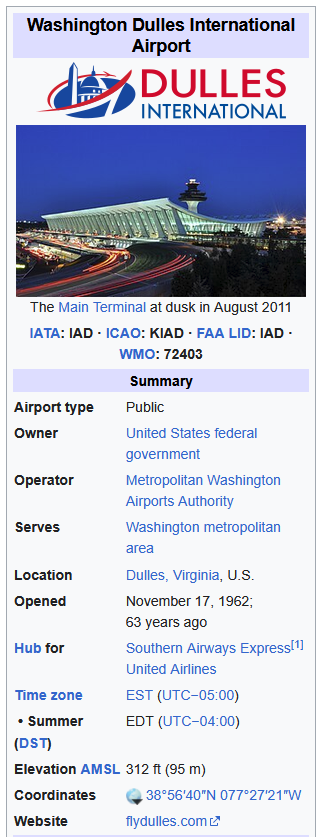
\includegraphics[height=0.65\textheight]{../../pics/airport_dulles_1.png}}}$%
  \hspace{0.75cm}%
  $\vcenter{\hbox{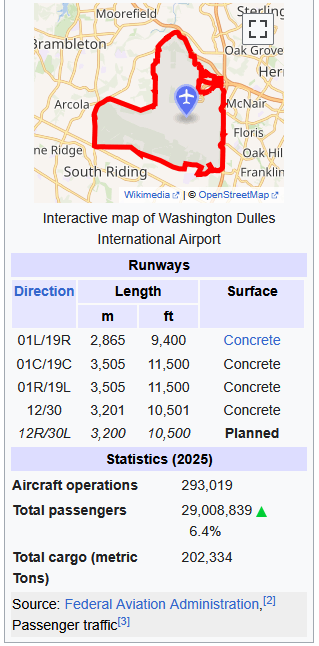
\includegraphics[height=0.65\textheight]{../../pics/airport_dulles_2.png}}}$%
  \hspace{0.75cm}%
  % crop to the runway table: trim = left bottom right top (in bp)
  $\vcenter{\hbox{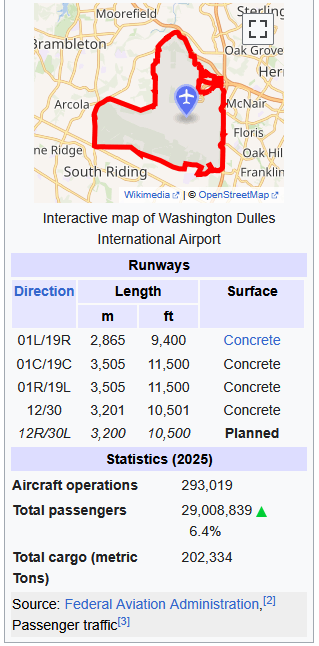
\includegraphics[width=0.4\textwidth, trim=0 99 0 125, clip]{../../pics/airport_dulles_2.png}}}$
\end{center}
\vspace{5mm}
\begin{center}
\scriptsize \url{https://en.wikipedia.org/wiki/Dulles_International_Airport}
\end{center}
\end{frame}


\section{Vibecoding 1}

\begin{frame}[fragile]{Setting Up for Vibecoding}

We only need the airports that appear in \texttt{flights}, as origin or destination:
\begin{lstlisting}[language=R, basicstyle=\ttfamily\small]
# Keep only the airports that appear in flights, as origin or destination
airports <- airports[airports$faa %in% c(flights$origin, flights$dest), ]
nrow(airports)
head(airports$faa)
\end{lstlisting}
\begin{lstlisting}[language=R, basicstyle=\ttfamily\small]
> nrow(airports)
[1] 103
> head(airports$faa)
[1] "ABQ" "ACK" "ALB" "ANC" "ATL" "AUS"
\end{lstlisting}
\end{frame}

\begin{frame}{The LLM Prompt}
\linespread{1.3}\selectfont % dense slide: tighter line spacing so it fits

Ask your LLM of choice to write the scraper:

\begin{block}{}
\textit{I am working on R. I have a list of unique airport codes from the flights dataset \texttt{airports\$faa}, with elements of the list that look as follows: "ABQ" "ACK" "ALB" "ANC" "ATL" "AUS"... I want to extract information about each airport from its Wikipedia page. Write an R script that loops through the list, scrapes the Wikipedia pages (e.g., \url{https://en.wikipedia.org/wiki/} + airport code), extracts: 1) the number of runways in the airport, 2) the length of each runway, in metres, from the Wikipedia infobox.}
\end{block}

\pause
\begin{itemize}
  \item A minimal version of the resulting scraper uses \texttt{rvest}.
  \item Airports whose page is not found are skipped.
  \item Runway lengths are stored as a single text, separated by semicolons.
  \item Outcome: \texttt{df\_airports\_wiki} dataset.
\end{itemize}
\end{frame}

\begin{frame}[fragile]{The First Vibecoded Scraper}
\begin{lstlisting}[language=R, basicstyle=\ttfamily\tiny]
library(rvest)

# Empty dataframe to store the results, one row per airport
df_airports_wiki <- data.frame()

for (code in airports$faa) {

  # Read the Wikipedia page of the airport code; skip the code if the page does not exist
  page <- tryCatch(read_html(paste0("https://en.wikipedia.org/wiki/", code)),
                   error = function(e) NULL)
  if (is.null(page)) next

  # Rows of the runway table, inside the infobox at the top right of the page
  rows <- html_text2(html_elements(page, "table.infobox table tr"))

  # Runway rows start with a runway direction, e.g. "4L/22R  3,353  11,000  Asphalt"
  runways <- strsplit(rows[grepl("^[0-9]+[LCR]?/[0-9]+", rows)], "\t")

  # Lengths in metres: 2nd column, or 3rd if the table lists feet first
  m_col     <- if ("ft\tm" %in% rows) 3 else 2
  lengths_m <- sapply(runways, function(r) r[m_col])

  df_airports_wiki <- rbind(df_airports_wiki, data.frame(
    airport_code    = code,
    n_runways       = length(runways),
    runway_length_m = paste(lengths_m, collapse = "; ")
  ))

  Sys.sleep(0.5) # wait half a second between pages, to be polite to Wikipedia
}
\end{lstlisting}
\end{frame}

\begin{frame}[fragile]{Checking \texttt{df\_airports\_wiki}}

Coverage of the \texttt{n\_runways} variable seems to be perfect\dots
\begin{lstlisting}[language=R, basicstyle=\ttfamily\scriptsize]
> table(is.na(df_airports_wiki$n_runways))
FALSE
  103
\end{lstlisting}
\pause
\dots but is it?
\begin{lstlisting}[language=R, basicstyle=\ttfamily\scriptsize]
> table(df_airports_wiki$n_runways)
 0  1  2  3  4  5  6  8
85  2  5  2  6  1  1  1
\end{lstlisting}
\pause
\alert{85 of the 103 airports have 0 runways.} Only a few airports are properly recorded:
\begin{lstlisting}[language=R, basicstyle=\ttfamily\scriptsize]
> head(df_airports_wiki[df_airports_wiki$n_runways != 0, ])
   airport_code n_runways                          runway_length_m
8           BDL         2                             2,899; 2,087
19          CAK         2                             2,317; 2,501
32          DTW         6 3,659; 3,048; 3,048; 2,591; 2,654; 2,591
33          EGE         1                                    2,743
\end{lstlisting}
\end{frame}

\begin{frame}[fragile]{Sanity Check: Dulles International Airport}
\linespread{1.3}\selectfont % dense slide: tighter line spacing so it fits

\begin{columns}[c]
  \begin{column}{0.5\textwidth}
  Check the output against a case study.
  \begin{itemize}
    \item Washington Dulles International Airport (IAD) 
    \item \textbf{4 runways}: 3,505; 3,505; 3,200; 3,200 metres.
  \end{itemize}
  Did the scraper get it right?
  \end{column}
  \begin{column}{0.45\textwidth}
  \centering
  % crop to the runway table: trim = left bottom right top (in bp)
  $\vcenter{\hbox{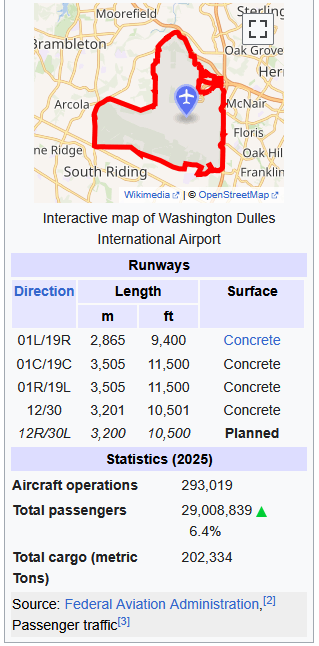
\includegraphics[width=\linewidth, trim=0 99 0 125, clip]{../../pics/airport_dulles_2.png}}}$
  \end{column}
\end{columns}
\pause
\vspace{3mm}
\begin{lstlisting}[language=R, basicstyle=\ttfamily\small]
> print(df_airports_wiki[df_airports_wiki$airport_code == "IAD", ])
   airport_code n_runways runway_length_m
43          IAD         0
\end{lstlisting}
\pause
\begin{center}
\alert{According to the scraper, Dulles has no runways.}
\end{center}
\end{frame}

\begin{frame}{Lesson from the First Attempt}

\begin{itemize}
  \item The vibecoded scraper recorded the runway information for a \textbf{few airports}\dots
  \item \dots but \textbf{most airports} were not recorded properly.
\end{itemize}

\pause
\begin{block}{Danger: the failure is easy to miss}
\begin{itemize}
  \item Even when the scraper found no information, it filled in \texttt{n\_runways} with 0.
  \item Every airport has a value: at first glance, the scraper seems to have done a great job.
\end{itemize}
\end{block}

\pause
\begin{center}
\alert{A script that runs without errors and returns a complete dataset is not necessarily correct.}
\end{center}
\end{frame}


\section{Vibecoding 2}

\begin{frame}[fragile]{Refining the Prompt}
\linespread{1.3}\selectfont % dense slide: tighter line spacing so it fits

List the airports that were not found in the first attempt:
\begin{lstlisting}[language=R, basicstyle=\ttfamily\tiny]
> df_airports_not_found <- df_airports_wiki$airport_code[df_airports_wiki$n_runways == 0]
> print(df_airports_not_found)
 [1] "ABQ" "ACK" "ALB" "ANC" "ATL" "AUS" "AVL" "BGR" "BHM" "BNA" "BOS" "BTV"
[13] "BUF" "BUR" "BWI" "BZN" "CAE" "CHO" "CHS" "CLE" "CLT" "CMH" "CRW" "CVG"
...
[85] "XNA"
\end{lstlisting}
\pause
Generate a new prompt, asking the LLM to improve the scraper:
\begin{block}{}
\textit{The previous scraper missed the following airports: [paste the list of missed airports here]. Moreover, I want that, if you are unable to find a specific variable, such as the number of runways \texttt{n\_runways}, you record "NA" instead of 0. If the number of runways is NA, record the runway length variable \texttt{runway\_length\_m} as "NA". Generate a new version of the scraper.}
\end{block}
\end{frame}

\begin{frame}[fragile]{What Changed in the Scraper}
\linespread{1.3}\selectfont % dense slide: tighter line spacing so it fits

\textcolor{teal}{New 1}: instead of guessing the page address, ask Wikipedia's search engine for ``\textit{code} airport'' and take the title of the first result:
\begin{lstlisting}[language=R, basicstyle=\ttfamily\tiny]
search_url <- paste0("https://en.wikipedia.org/w/api.php?action=query&list=search",
                     "&format=json&srsearch=", code, "%20airport")
title <- tryCatch(content(GET(search_url))$query$search[[1]]$title,
                  error = function(e) NULL)
page <- if (is.null(title)) NULL else
  tryCatch(read_html(paste0("https://en.wikipedia.org/wiki/", URLencode(title))),
           error = function(e) NULL)
\end{lstlisting}
\pause
\textcolor{teal}{New 2}: if the page is not found, keep the airport in the dataset with \texttt{NA} values:
\begin{lstlisting}[language=R, basicstyle=\ttfamily\tiny]
if (is.null(page)) {
  df_airports_wiki2 <- rbind(df_airports_wiki2, data.frame(
    airport_code = code, airport_name = NA, n_runways = NA, runway_length_m = NA))
  next
}
\end{lstlisting}
\pause
\textcolor{teal}{New 3}: \texttt{NA} instead of 0 if no runways are found, and then also \texttt{NA} for their lengths:
\begin{lstlisting}[language=R, basicstyle=\ttfamily\tiny]
n_runways       <- if (length(runways) == 0) NA else length(runways)
runway_length_m <- if (is.na(n_runways)) NA else paste(lengths_m, collapse = "; ")
\end{lstlisting}
The rest of the scraper (runway table, lengths in metres) is unchanged.
\end{frame}

\begin{frame}[fragile]{Results of the Second Attempt}

\begin{columns}[t]
  \begin{column}{0.5\textwidth}
\begin{lstlisting}[language=R, basicstyle=\ttfamily\scriptsize]
> head(df_airports_wiki2)
  airport_code n_runways     runway_length_m
1          ABQ         3 3,048; 4,204; 1,829
2          ACK         2        1,921; 1,372
3          ALB         2        2,591; 2,195
4          ANC         3 3,780; 3,312; 3,231
\end{lstlisting}
  \end{column}
  \begin{column}{0.45\textwidth}
\begin{lstlisting}[language=R, basicstyle=\ttfamily\scriptsize]
> table(is.na(df_airports_wiki2$n_runways))
FALSE
  103
> table(df_airports_wiki2$n_runways)
 1  2  3  4  5  6  7  8
12 36 27 19  4  3  1  1
\end{lstlisting}
  \end{column}
\end{columns}

\pause
No more airports with 0 runways. Sanity check: what about Dulles?
\begin{lstlisting}[language=R, basicstyle=\ttfamily\scriptsize]
> print(df_airports_wiki2[df_airports_wiki2$airport_code == "IAD",
+                         c("airport_code", "n_runways", "runway_length_m")])
   airport_code n_runways                   runway_length_m
43          IAD         5 2,865; 3,505; 3,505; 3,201; 3,200
\end{lstlisting}
\pause
\begin{center}
\alert{Much better, but is it right? Compare with the Wikipedia infobox.}
\end{center}
\end{frame}


\section{Final Dataset}

\begin{frame}[fragile]{Merging Twice: Airport of Origin}
\linespread{1.3}\selectfont % dense slide: tighter line spacing so it fits

\begin{itemize}
  \item \texttt{df\_airports\_wiki2} is a complement: we merge it with the base dataset \texttt{flights}.
  \item Each flight involves two airports: merge \textbf{twice}, once for the origin and once for the destination.
  \item Rename the variables with the prefix \texttt{origin\_}, and the key as \texttt{origin}, as in \texttt{flights}:
\end{itemize}
\begin{columns}[t]
  \begin{column}{0.55\textwidth}
\begin{lstlisting}[language=R, basicstyle=\ttfamily\tiny]
library(dplyr)

# Airport information, referring to the airport of origin
df_origin <- df_airports_wiki2 |>
  select(origin                 = airport_code,
         origin_n_runways       = n_runways,
         origin_runway_length_m = runway_length_m)

df_flights <- flights |>
  left_join(df_origin, by = "origin")
\end{lstlisting}
  \end{column}
  \begin{column}{0.4\textwidth}
  \pause
  A left join keeps every flight (336,776 rows). Only three origin airports:
\begin{lstlisting}[language=R, basicstyle=\ttfamily\tiny]
> table(df_flights$origin,
+       df_flights$origin_n_runways)
           2      3      4
  EWR      0 120835      0
  JFK      0      0 111279
  LGA 104662      0      0
\end{lstlisting}
  \end{column}
\end{columns}
\end{frame}

\begin{frame}[fragile]{Merging Twice: Airport of Destination}

Same steps, with the prefix \texttt{dest\_}:
\begin{lstlisting}[language=R, basicstyle=\ttfamily\scriptsize]
# Airport information, referring to the airport of destination
df_dest <- df_airports_wiki2 |>
  select(dest                 = airport_code,
         dest_n_runways       = n_runways,
         dest_runway_length_m = runway_length_m)

df_flights <- df_flights |>
  left_join(df_dest, by = "dest")

dim(df_flights)   # 336776 rows, 23 columns
\end{lstlisting}
\pause
Coverage of the runway variables (rows: destination missing; columns: origin missing):
\begin{lstlisting}[language=R, basicstyle=\ttfamily\scriptsize]
> table(is.na(df_flights$dest_n_runways), is.na(df_flights$origin_n_runways))
         FALSE
  FALSE 329174
  TRUE    7602
\end{lstlisting}
\alert{7,602 flights have no information on the airport of destination.}
\end{frame}

\begin{frame}[fragile]{Saving the Dataset}

Save the enriched dataset to a CSV file for later use. Unless told otherwise, R saves it in the working directory:
\begin{lstlisting}[language=R, basicstyle=\ttfamily\small]
# Print the working directory
getwd()

# Save dataset df_flights
write.csv(df_flights, "data/df_flights_enriched.csv", row.names = FALSE)
\end{lstlisting}
\end{frame}


\section{Conclusion}

\begin{frame}{Summary}

\begin{block}{Today}
\begin{enumerate}
  \item Data from the web: direct download, APIs, web scraping.
  \item Vibecoding a scraper with an LLM, and \textbf{checking} its output: coverage tables, and a known case (Dulles).
  \item Refining the prompt until the output is reliable.
  \item Merging the scraped data with the base dataset, twice: origin and destination.
\end{enumerate}
\end{block}

\pause
\begin{center}
\alert{Never trust a dataset just because it looks complete.}
\end{center}

\pause
\textbf{Next class}: once our data is assembled and cleaned, we start exploring it with summary tables and visualizations of the relationships between economically relevant variables.
\end{frame}

\end{document}
